\chapter{Results and Discussion}

\section{PID}
\begin{figure}[!ht]
    \centering
    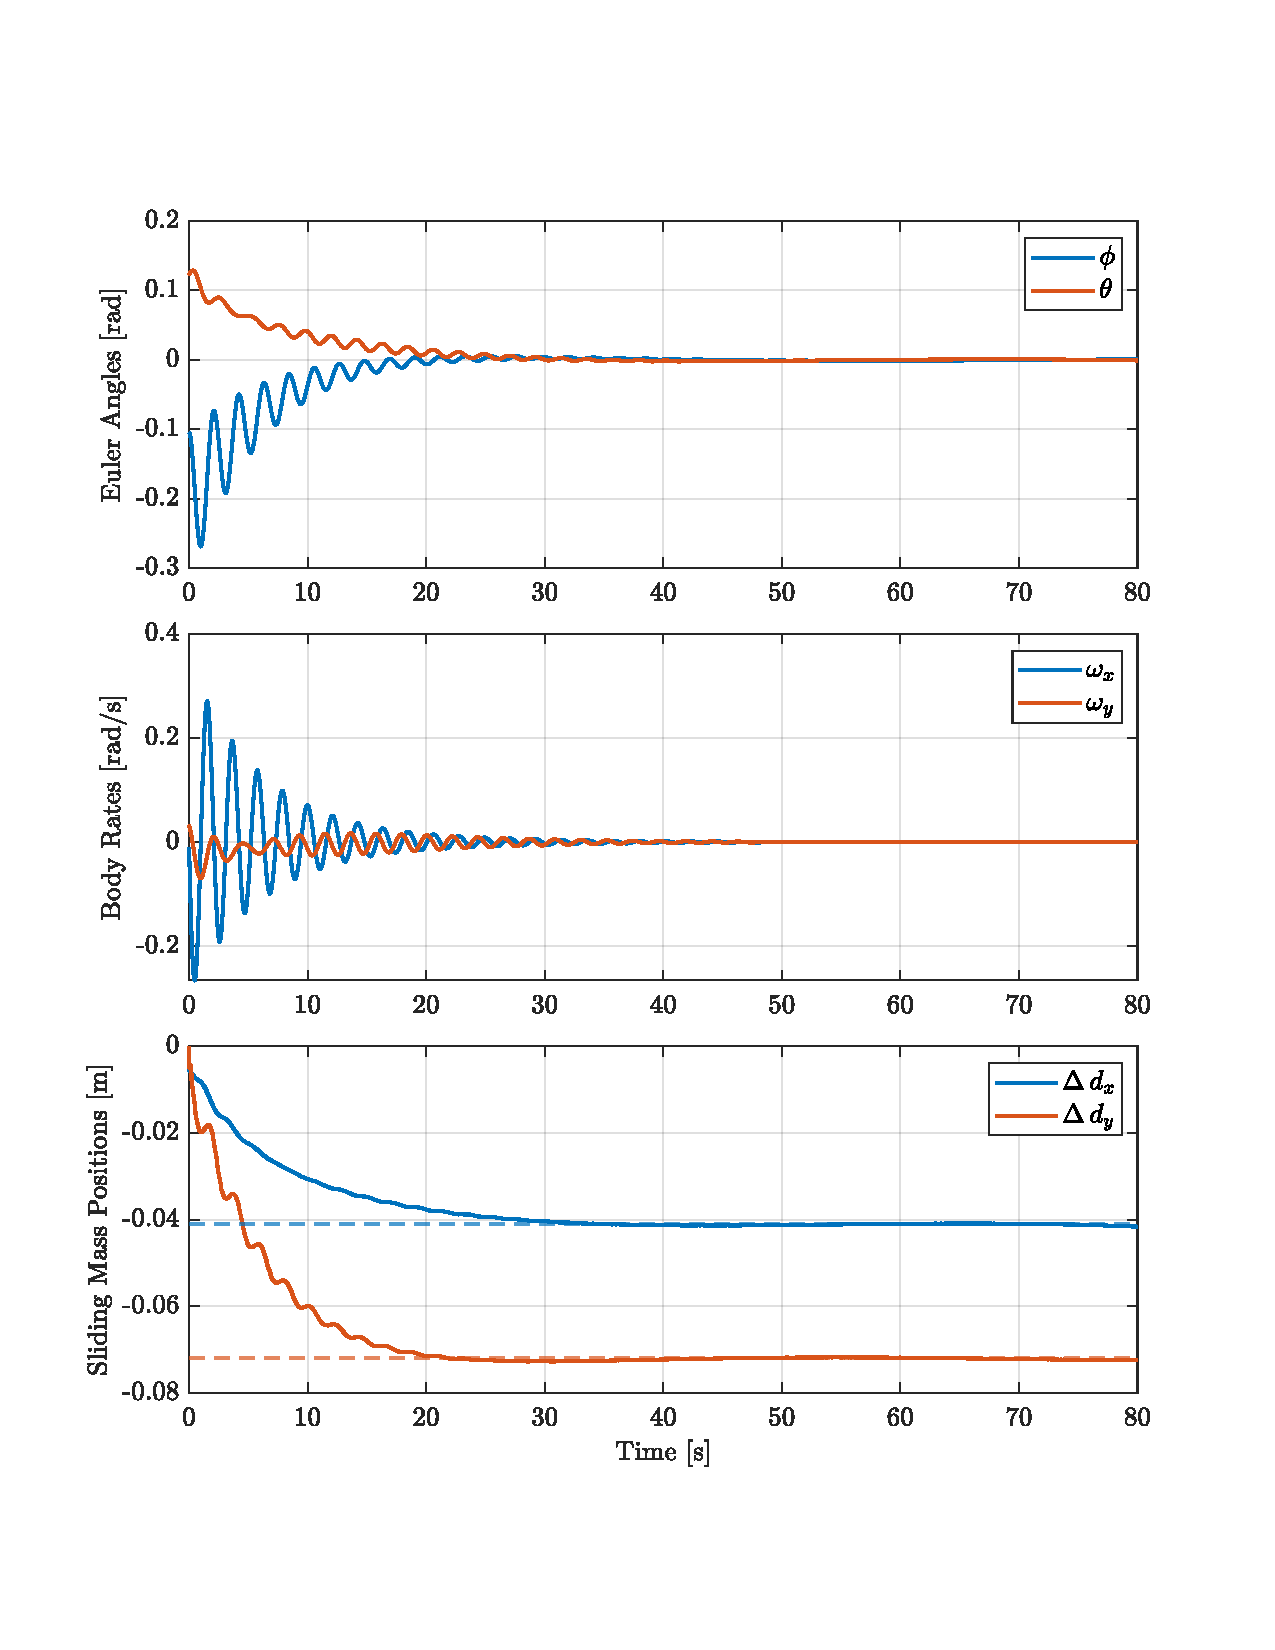
\includegraphics[width=\linewidth]{plots/PID_sim_results.pdf}
    \caption{Simulated balancing results using PID control}
\end{figure}

\begin{figure}[!ht]
    \centering
    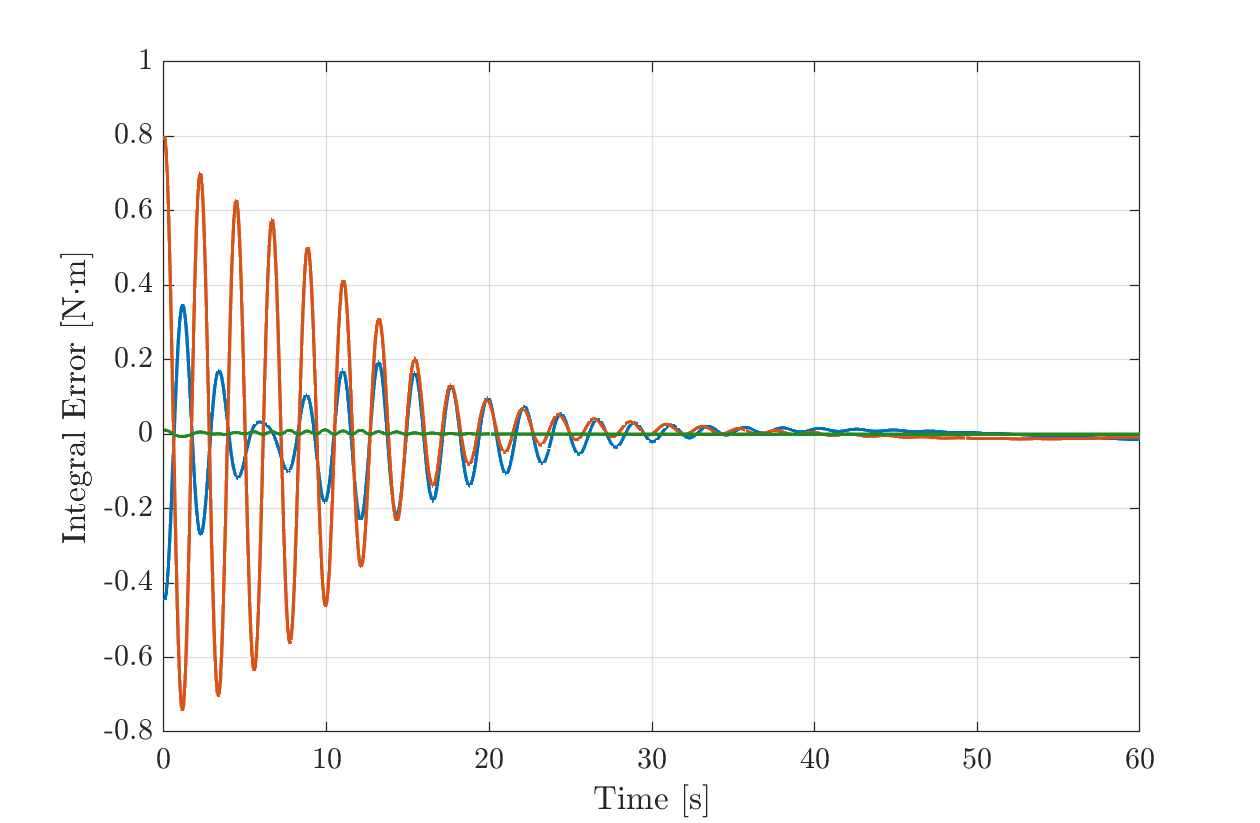
\includegraphics[width=\linewidth]{plots/PID_sim_integral_error.png}
    \caption{Projected integral error during a simulated PID run}
\end{figure}

\begin{figure}[!ht]
    \centering
    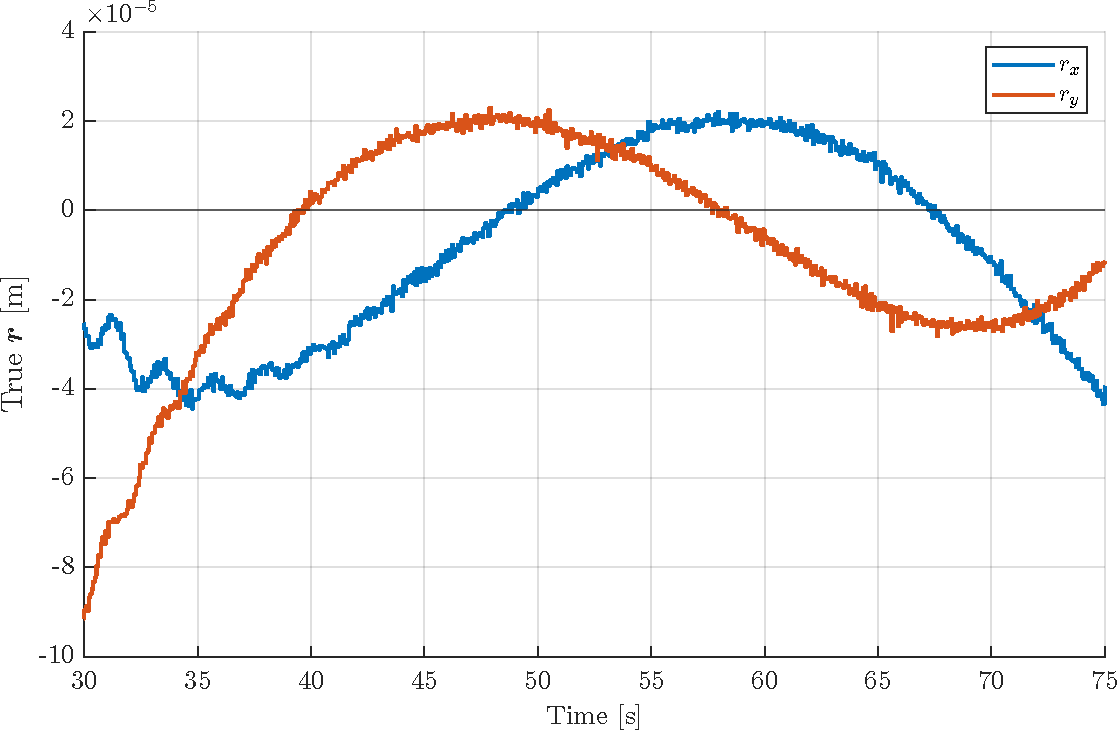
\includegraphics[width=\linewidth]{plots/PID_sim_oscillations.pdf}
    \caption{Simulated PID scillatations about $\bm{r}=0$ at steady state}
\end{figure}



\begin{figure}[!ht]
    \centering
    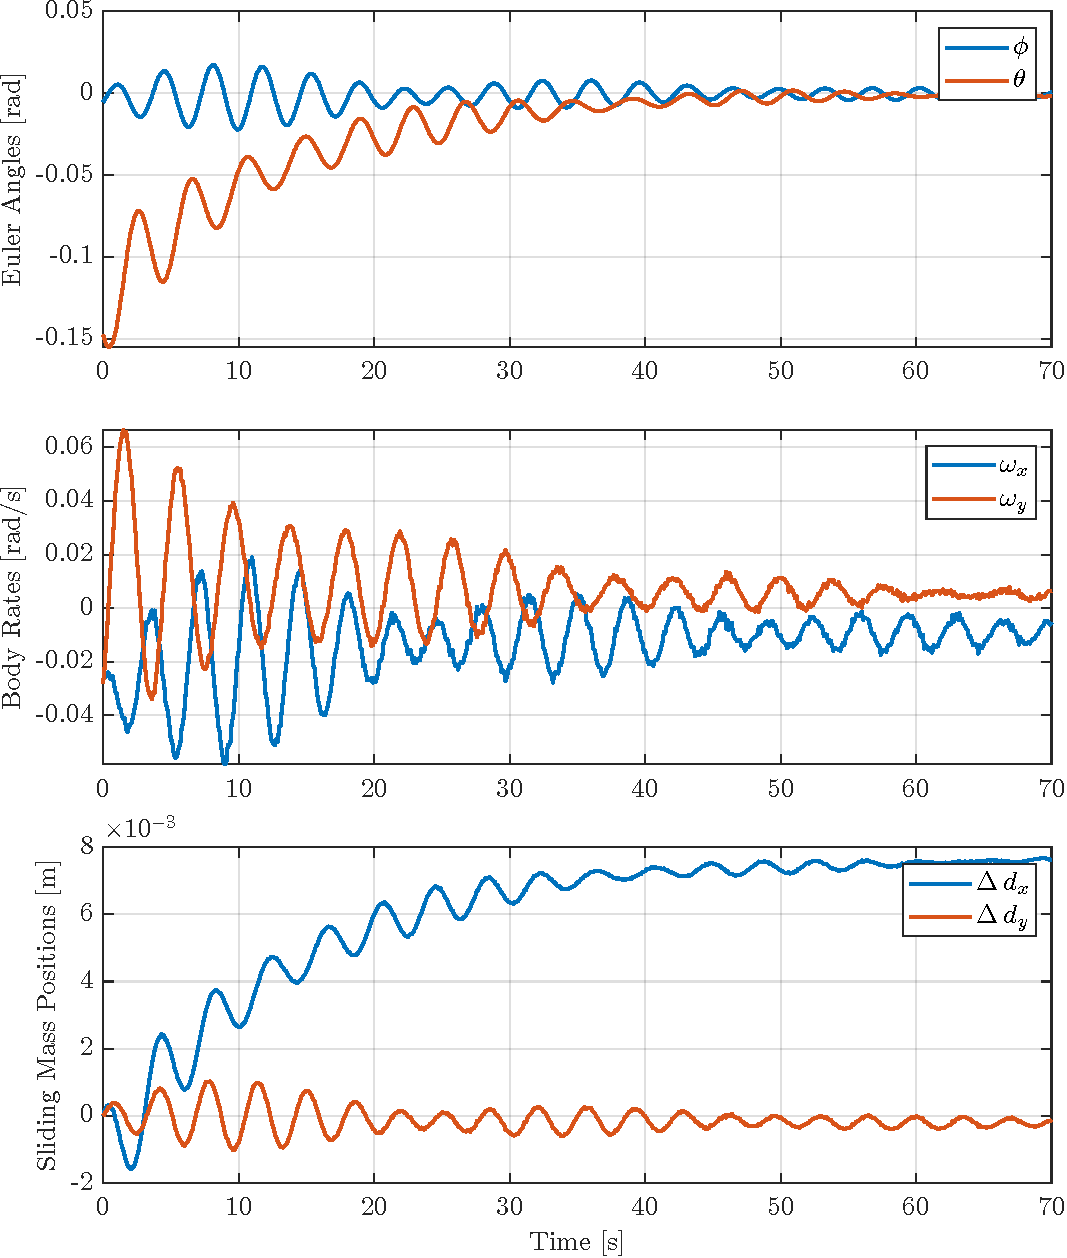
\includegraphics[width=\linewidth]{plots/PID_hardware_results.pdf}
    \caption{Experimental balancing results using PID control}
\end{figure}

\section{Underactuated Adaptive Control}

\begin{figure}[!ht]
    \centering
    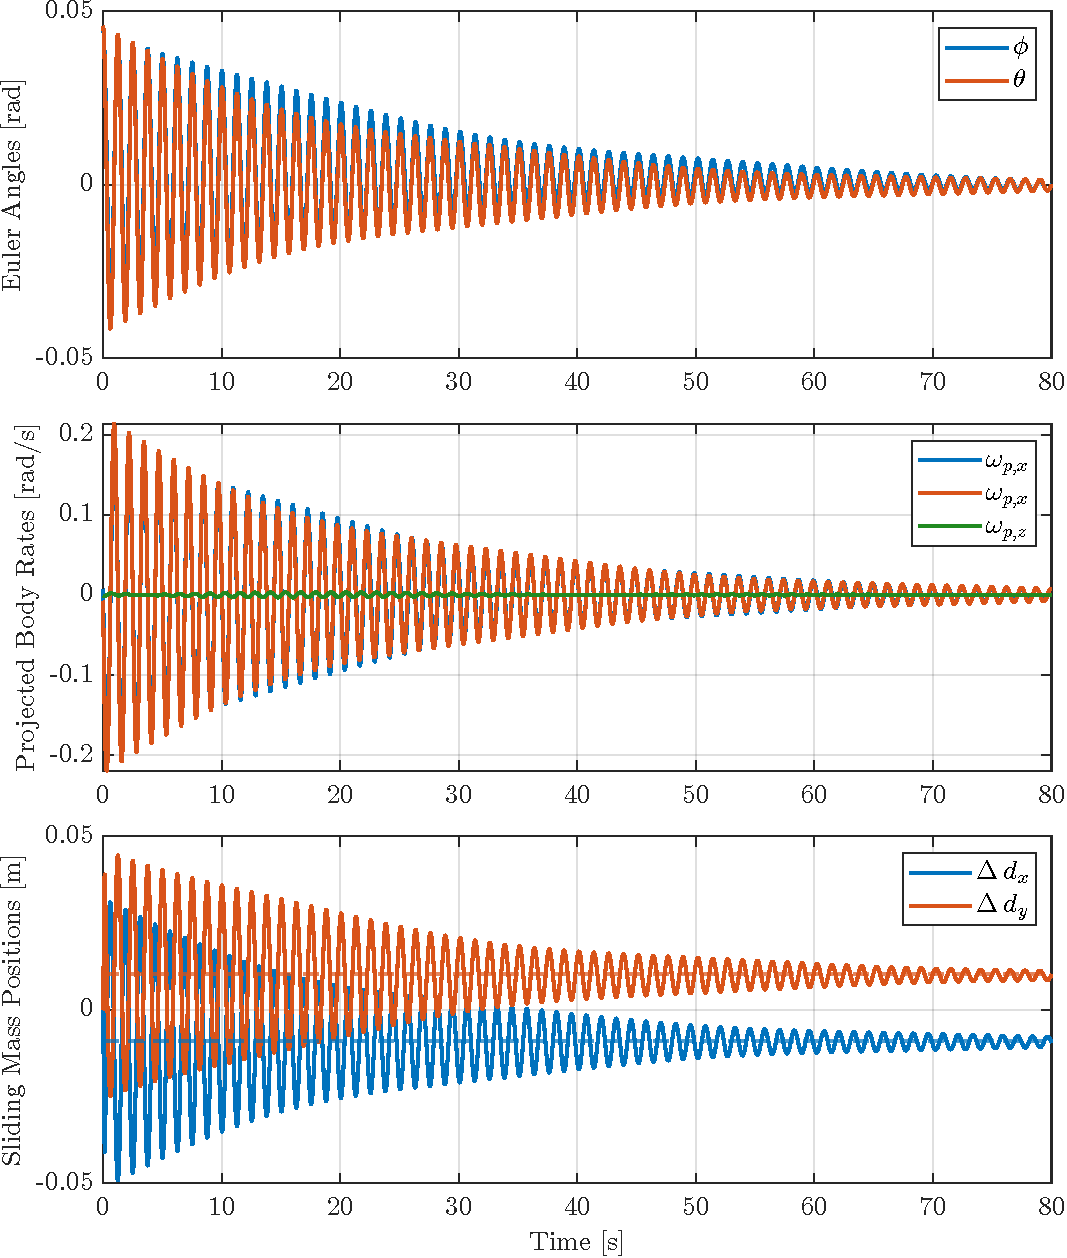
\includegraphics[width=\linewidth]{plots/adaptive_sim_success.pdf}
    \caption{Simulated underactuated adaptive control results using a simplified model}
\end{figure}

\begin{figure}[!ht]
    \centering
    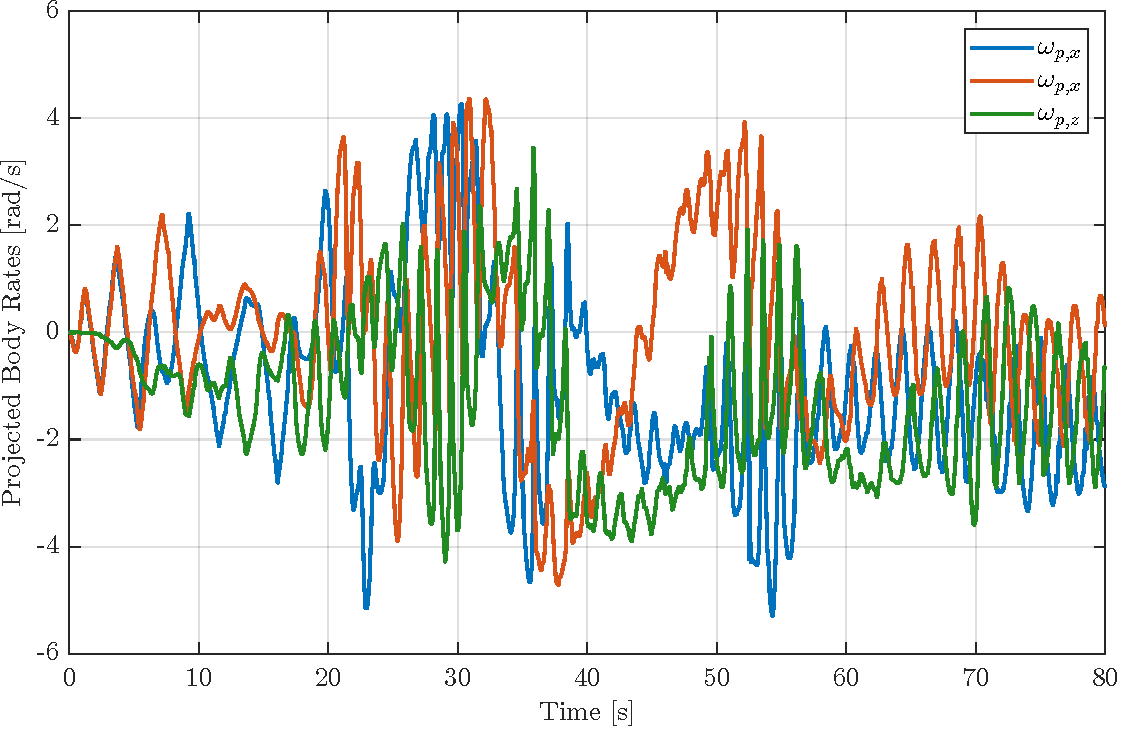
\includegraphics[width=\linewidth]{plots/adaptive_sim_failure.pdf}
    \caption{Simulated underactuated adaptive control results with sensor dyanmics and onboard filtering modeled}
\end{figure}

\begin{figure}[!ht]
    \centering
    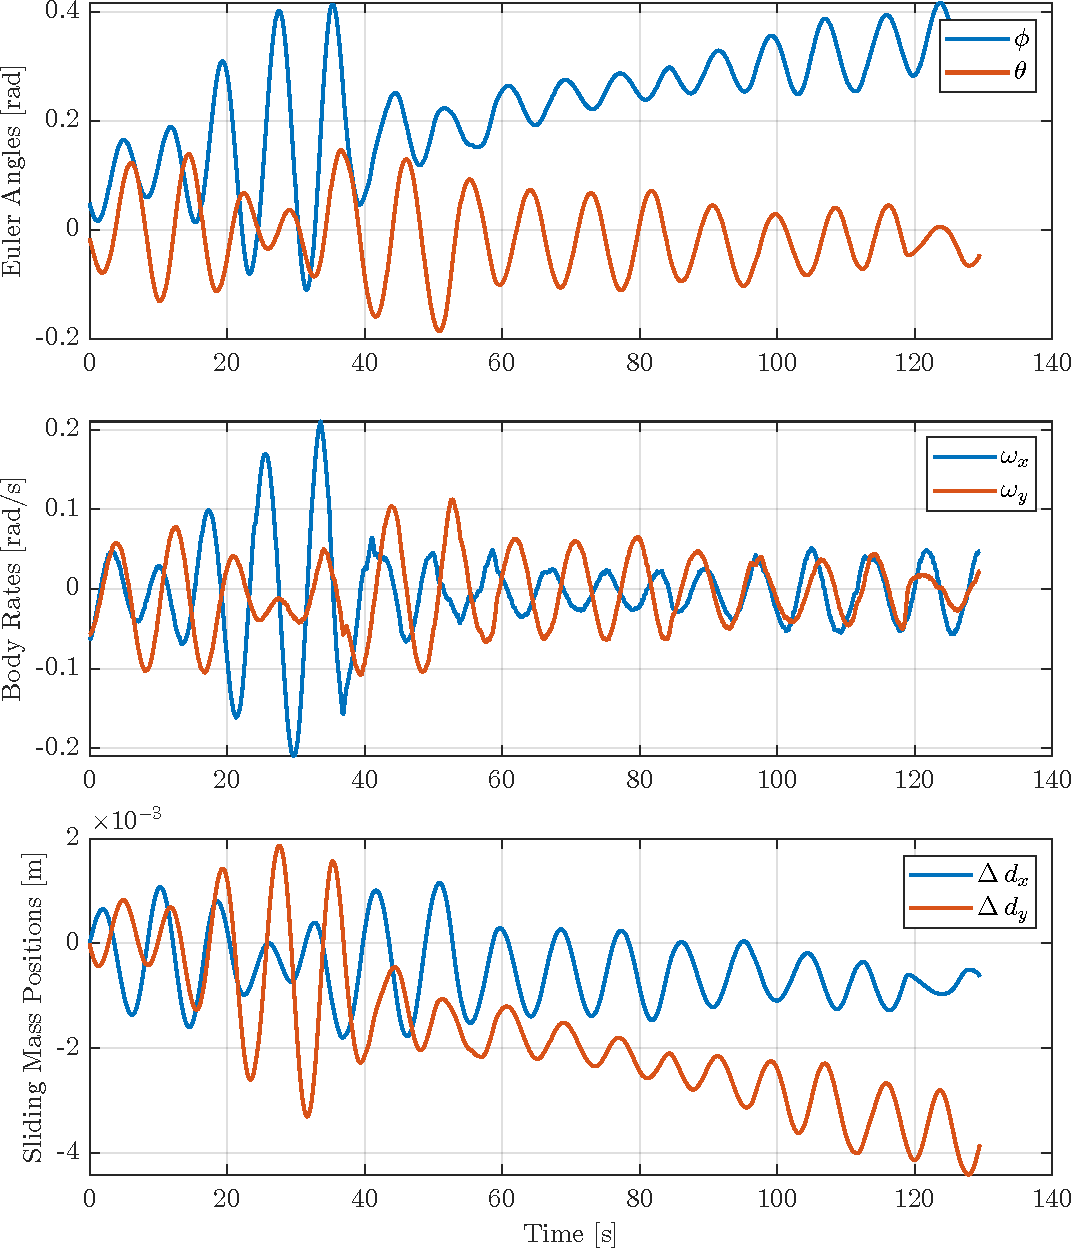
\includegraphics[width=\linewidth]{plots/adaptive_hardware_failure.pdf}
    \caption{Experimental results using underactuated adaptive control}
\end{figure}


\section{Vertical Inbalance Estimation with Kalman Filtering}

\begin{figure}[!ht]
  \centering
  \begin{subfigure}[t]{0.47\textwidth}
    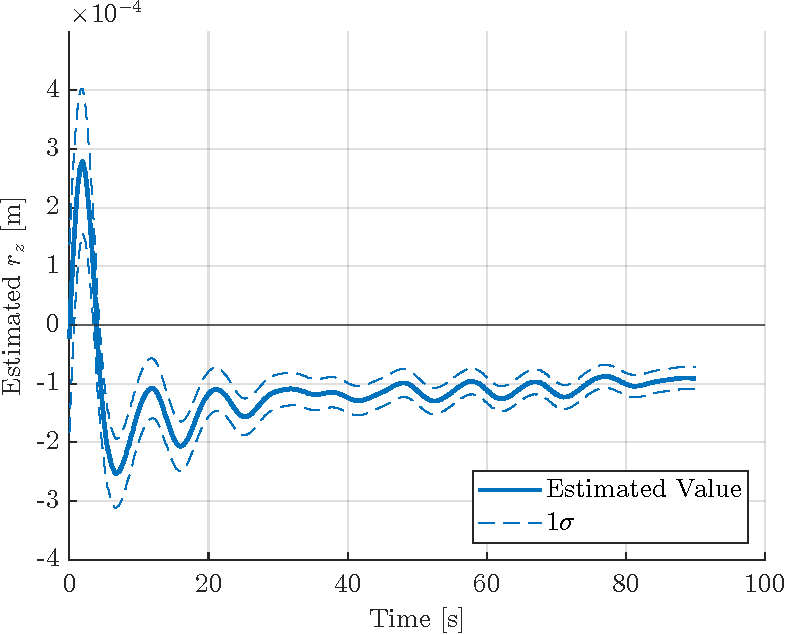
\includegraphics[width=\linewidth]{plots/UKF_hardware_success.pdf}
    \caption{Iteration successfully converging}\label{fig:a}
  \end{subfigure}\hfill
  \begin{subfigure}[t]{0.47\textwidth}
    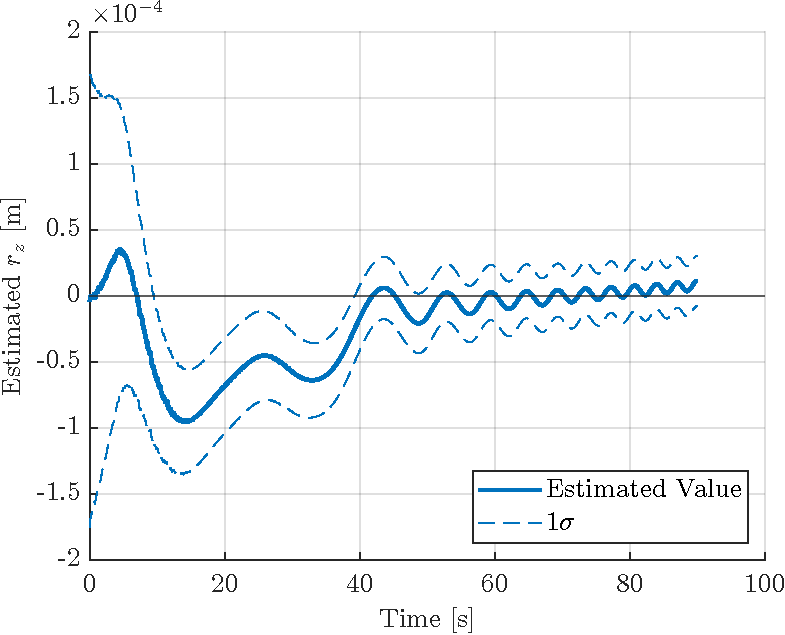
\includegraphics[width=\linewidth]{plots/UKF_hardware_failure.pdf}
    \caption{Iteration failing to converge}\label{fig:b}
  \end{subfigure}
  \caption{Experimental filter output during vertical inbalance estimation}
  \label{fig:twopanels}
\end{figure}

\begin{figure}[!ht]
  \centering
  \begin{subfigure}[t]{0.47\textwidth}
    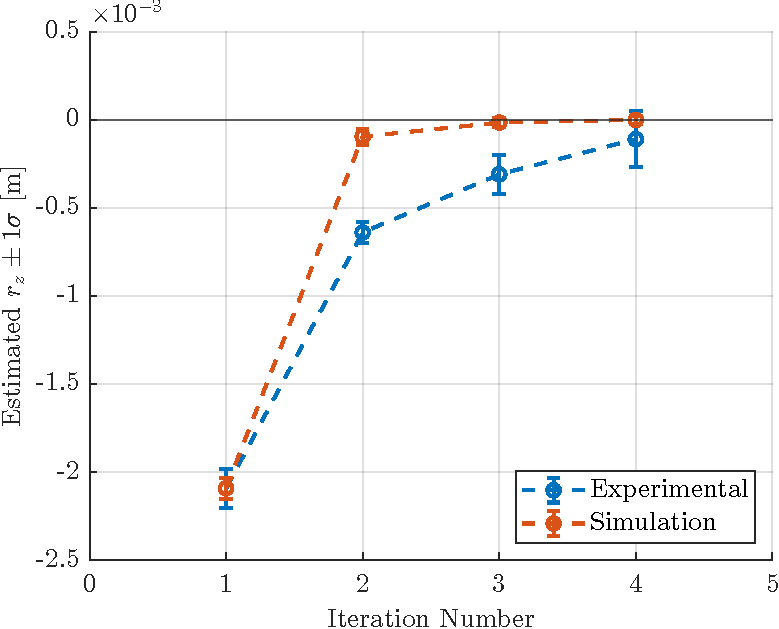
\includegraphics[width=\linewidth]{plots/UKF_comparison.pdf}
    \label{fig:a}
  \end{subfigure}\hfill
  \begin{subfigure}[t]{0.47\textwidth}
    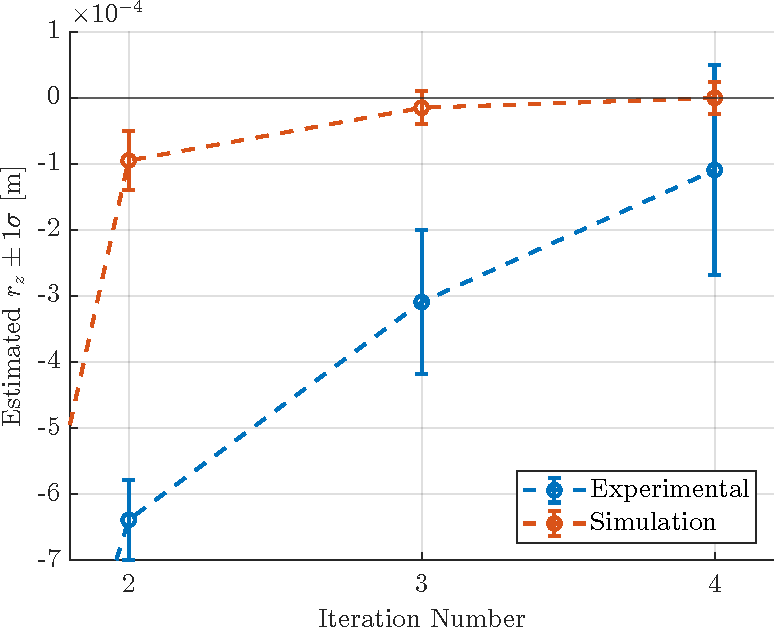
\includegraphics[width=\linewidth]{plots/UKF_comparison_zoomed.pdf}

    \label{fig:b}
  \end{subfigure}
  \caption{Filter results over multiple iterations, zoomed in on right}
  \label{fig:twopanels}
\end{figure}



\section{Passive Balancing Using Least-Squares Estimation}
% experimental results only use 1 RW
% simulation results should include 1 RW and 4 RWs to compare (unless the one RW setup turns out good)

\begin{figure}[!ht]
  \centering
  \begin{subfigure}[t]{0.47\textwidth}
    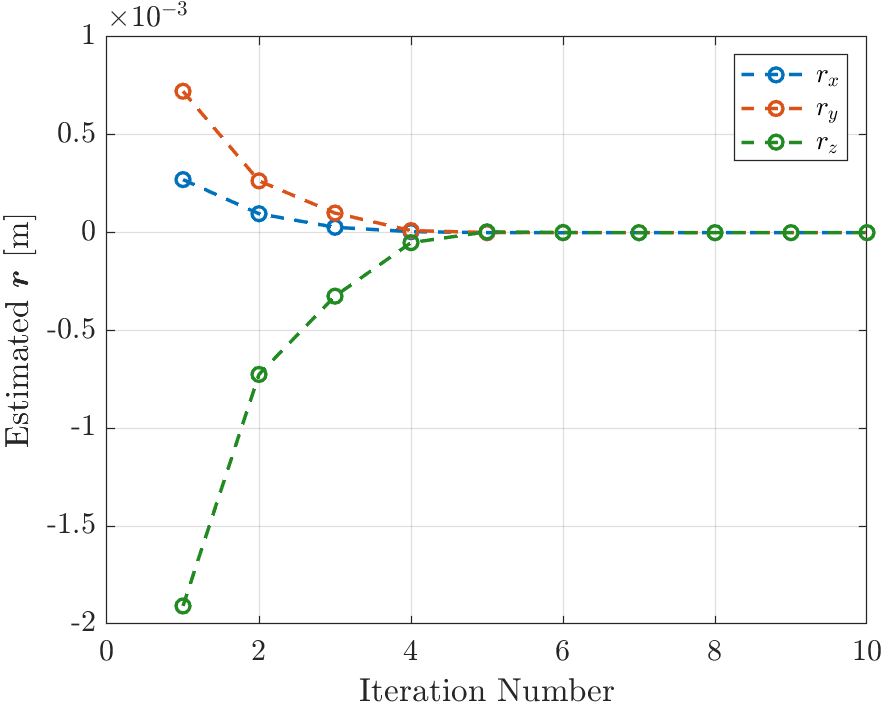
\includegraphics[width=\linewidth]{plots/LSR_sim_all_runs.png}
    \caption{All 10 iterations}\label{fig:a}
  \end{subfigure}\hfill
  \begin{subfigure}[t]{0.47\textwidth}
    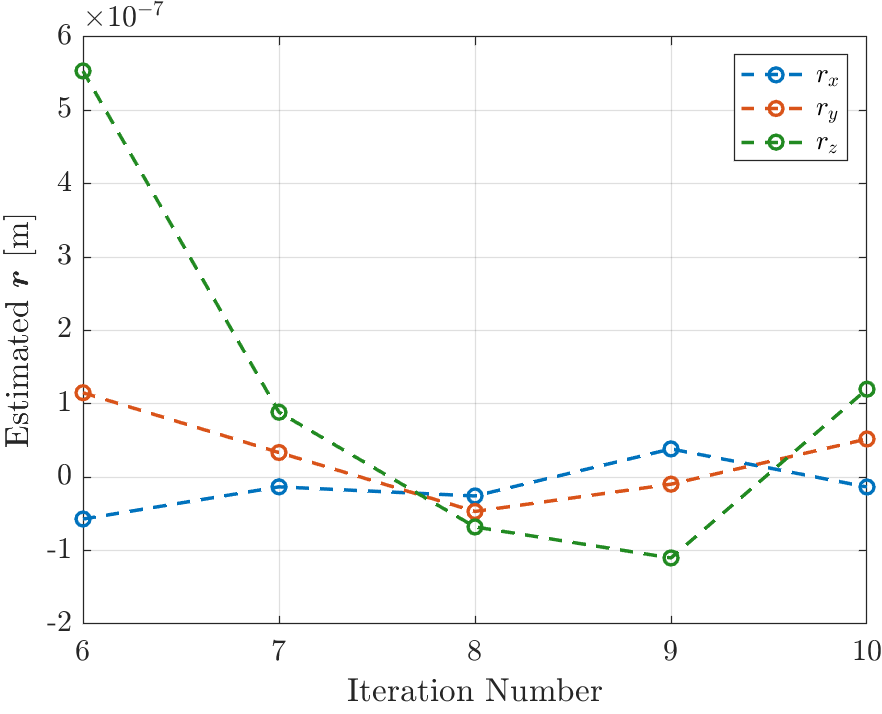
\includegraphics[width=\linewidth]{plots/LSR_sim_last_5_runs.png}
    \caption{Final 5 iterations}\label{fig:b}
  \end{subfigure}
  \caption{Simulated results of least-squares estimation method}
  \label{fig:twopanels}
\end{figure}

\begin{figure}[!ht]
    \centering
    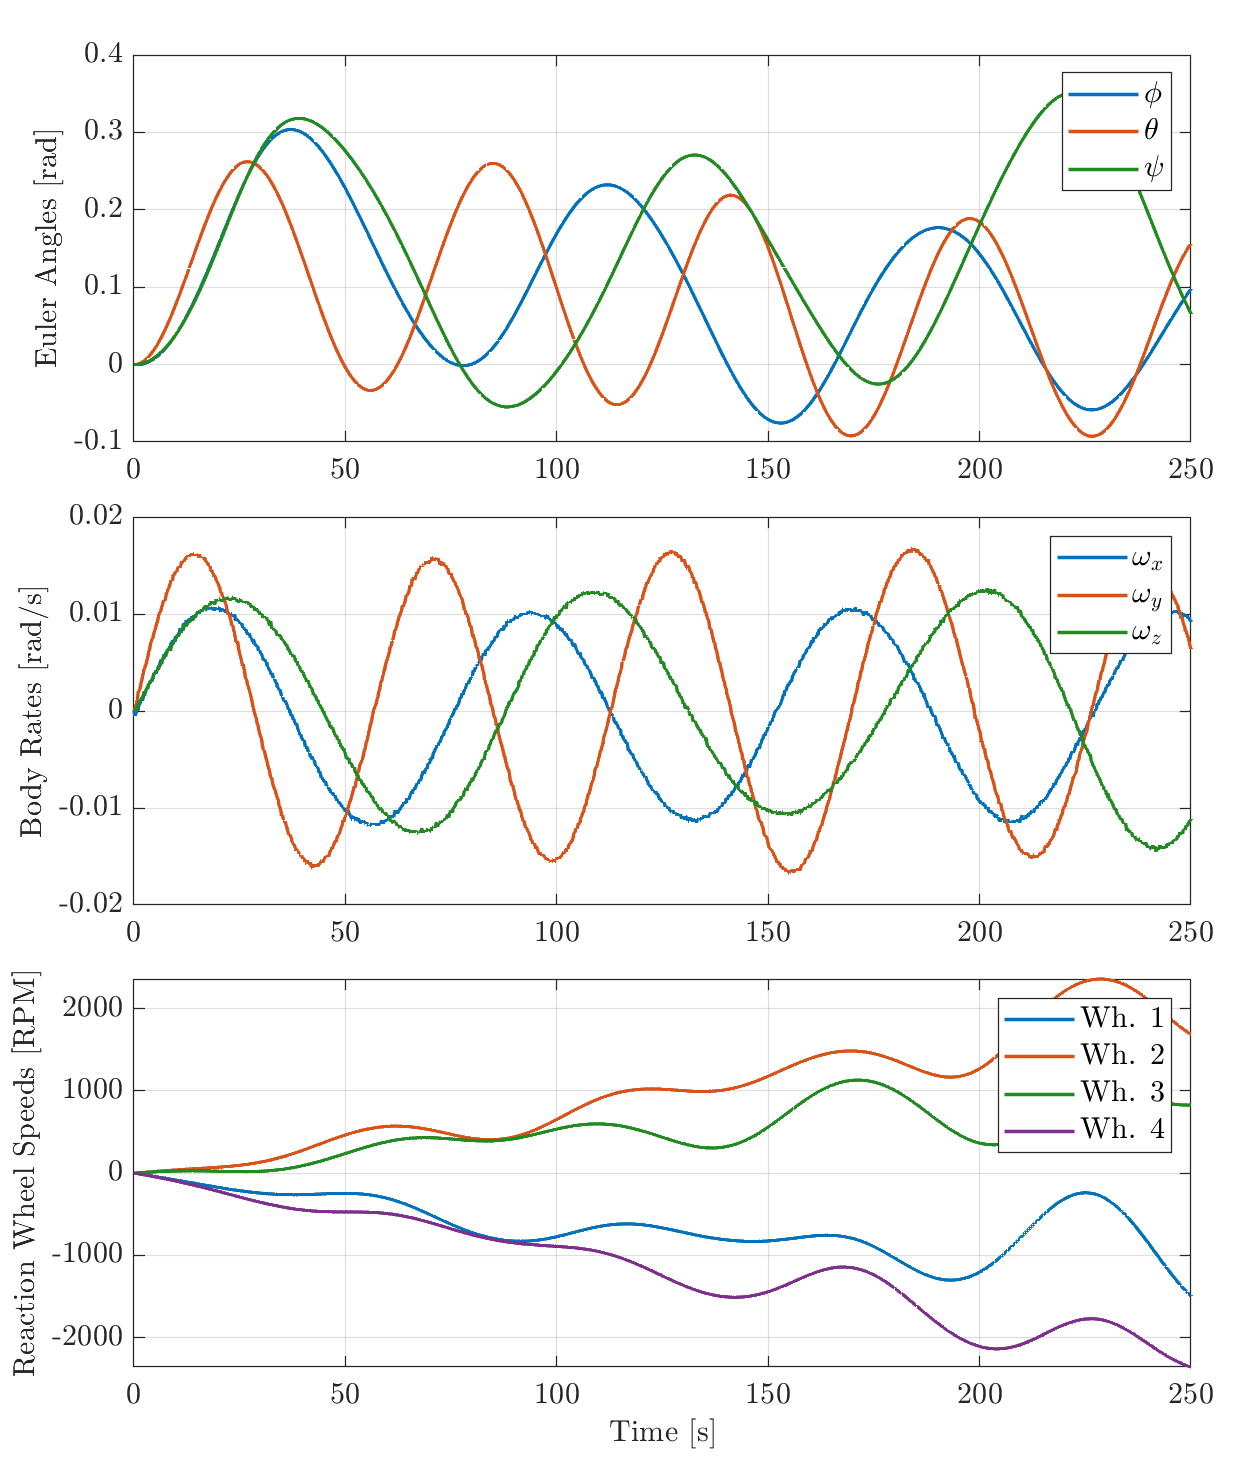
\includegraphics[width=\linewidth]{plots/LSR_sim_excitation}
    \caption{Simulated platform excitation during batch estimation}
\end{figure}

\begin{figure}[!ht]
  \centering
  \begin{subfigure}[t]{0.47\textwidth}
    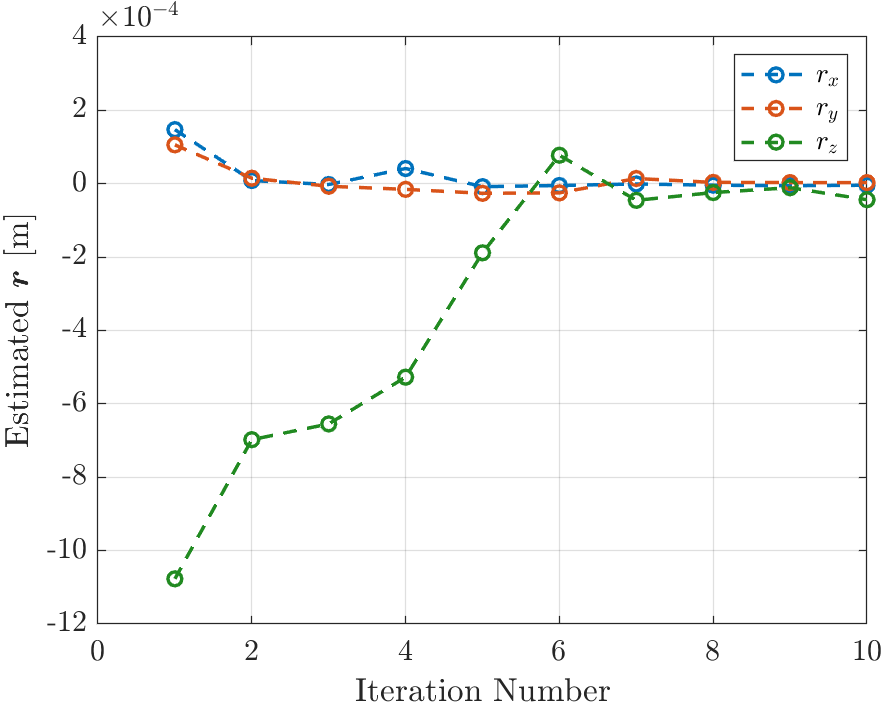
\includegraphics[width=\linewidth]{plots/LSR_hardware_all_runs.png}
    \caption{All 10 iterations}\label{fig:a}
  \end{subfigure}\hfill
  \begin{subfigure}[t]{0.47\textwidth}
    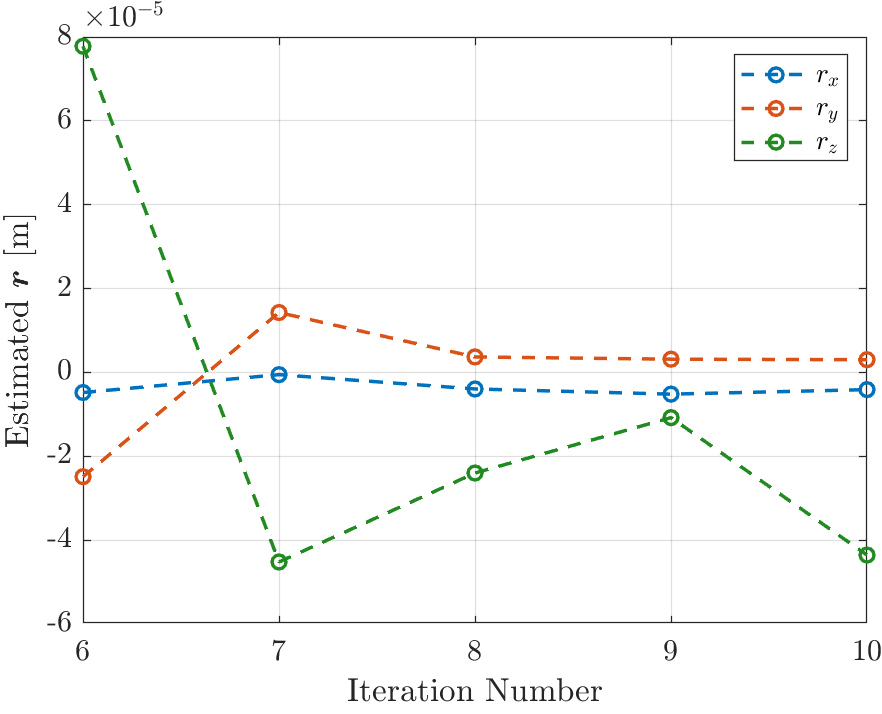
\includegraphics[width=\linewidth]{plots/LSR_hardware_last_5_runs.png}
    \caption{Final 5 iterations}\label{fig:b}
  \end{subfigure}
  \caption{Experimental results of least-squares estimation method}
  \label{fig:LSR_hardware_iterations}
\end{figure}

\begin{figure}[!ht]
    \centering
    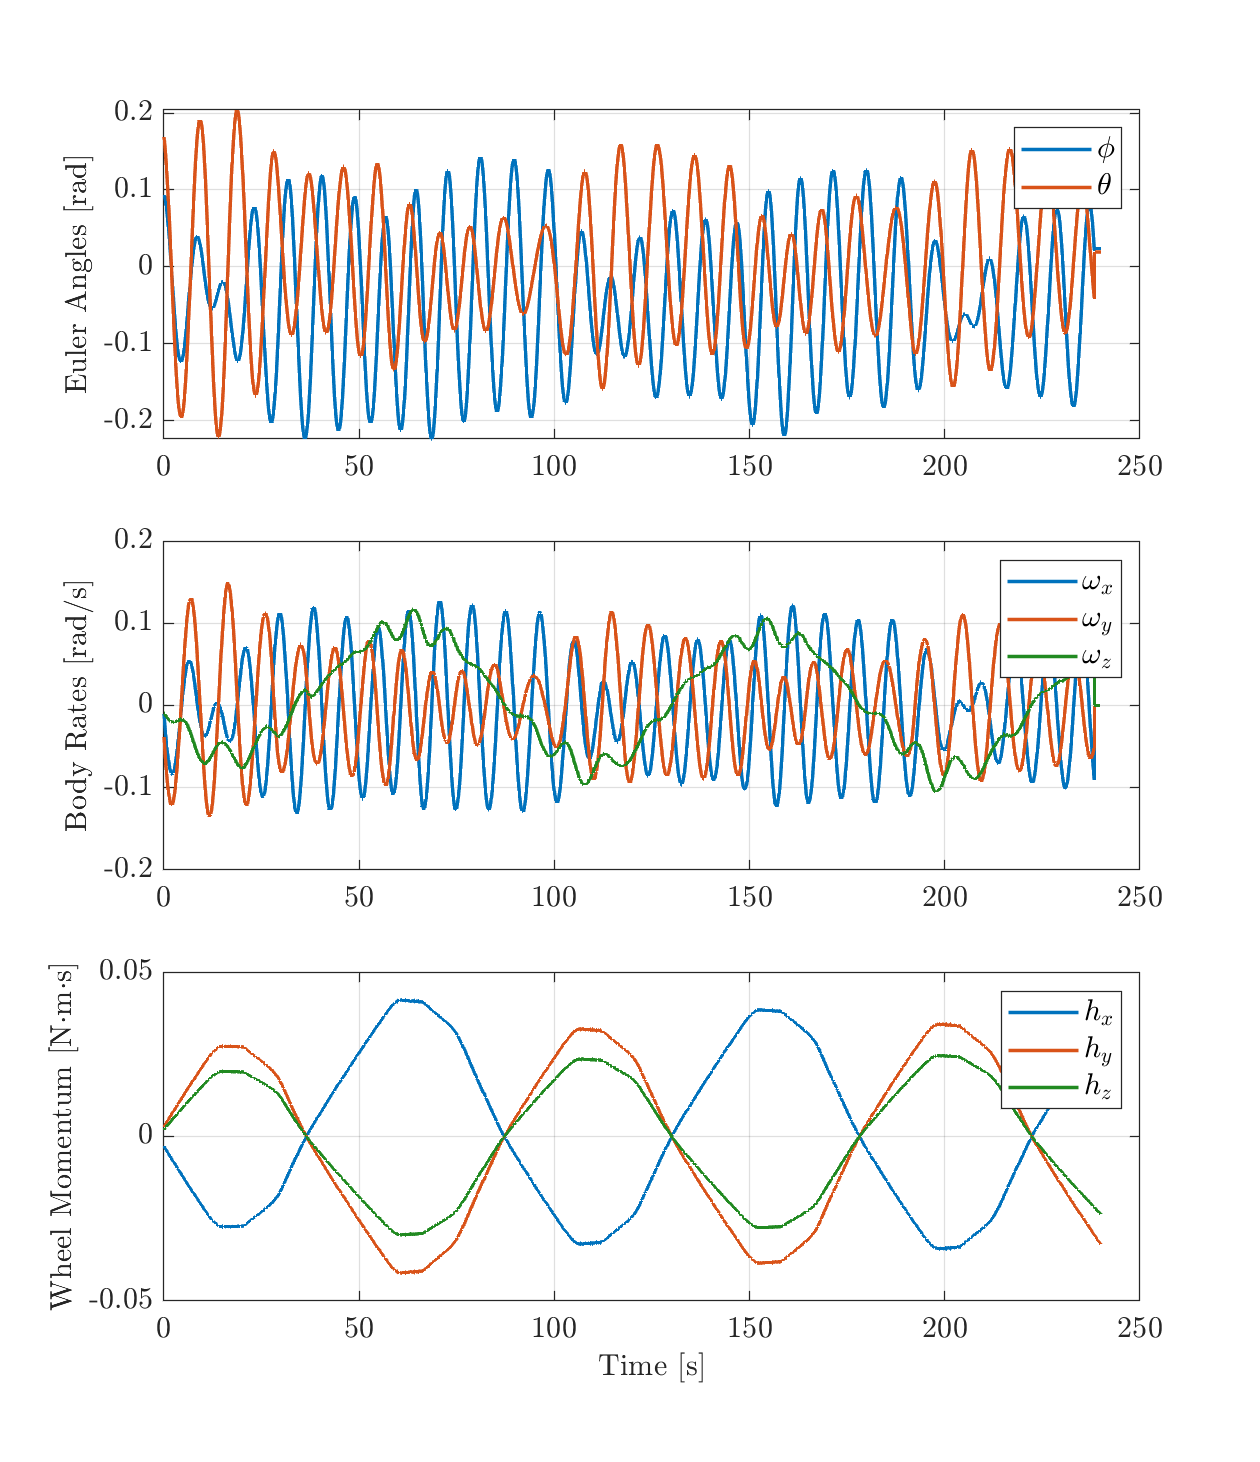
\includegraphics[width=\linewidth]{plots/LSR_hardware_excitation}
    \caption{Experimental platform excitation during batch estimation}
\end{figure}

\section{Active Balancing Using Adaptive Control}

\subsection{No Reaction Wheels}
% the experimental results for this are in a seperate repo - SADS Adaptive

\subsection{Full Reaction Wheel Setup - Simulink Only}

\begin{figure}[!ht]
    \centering
    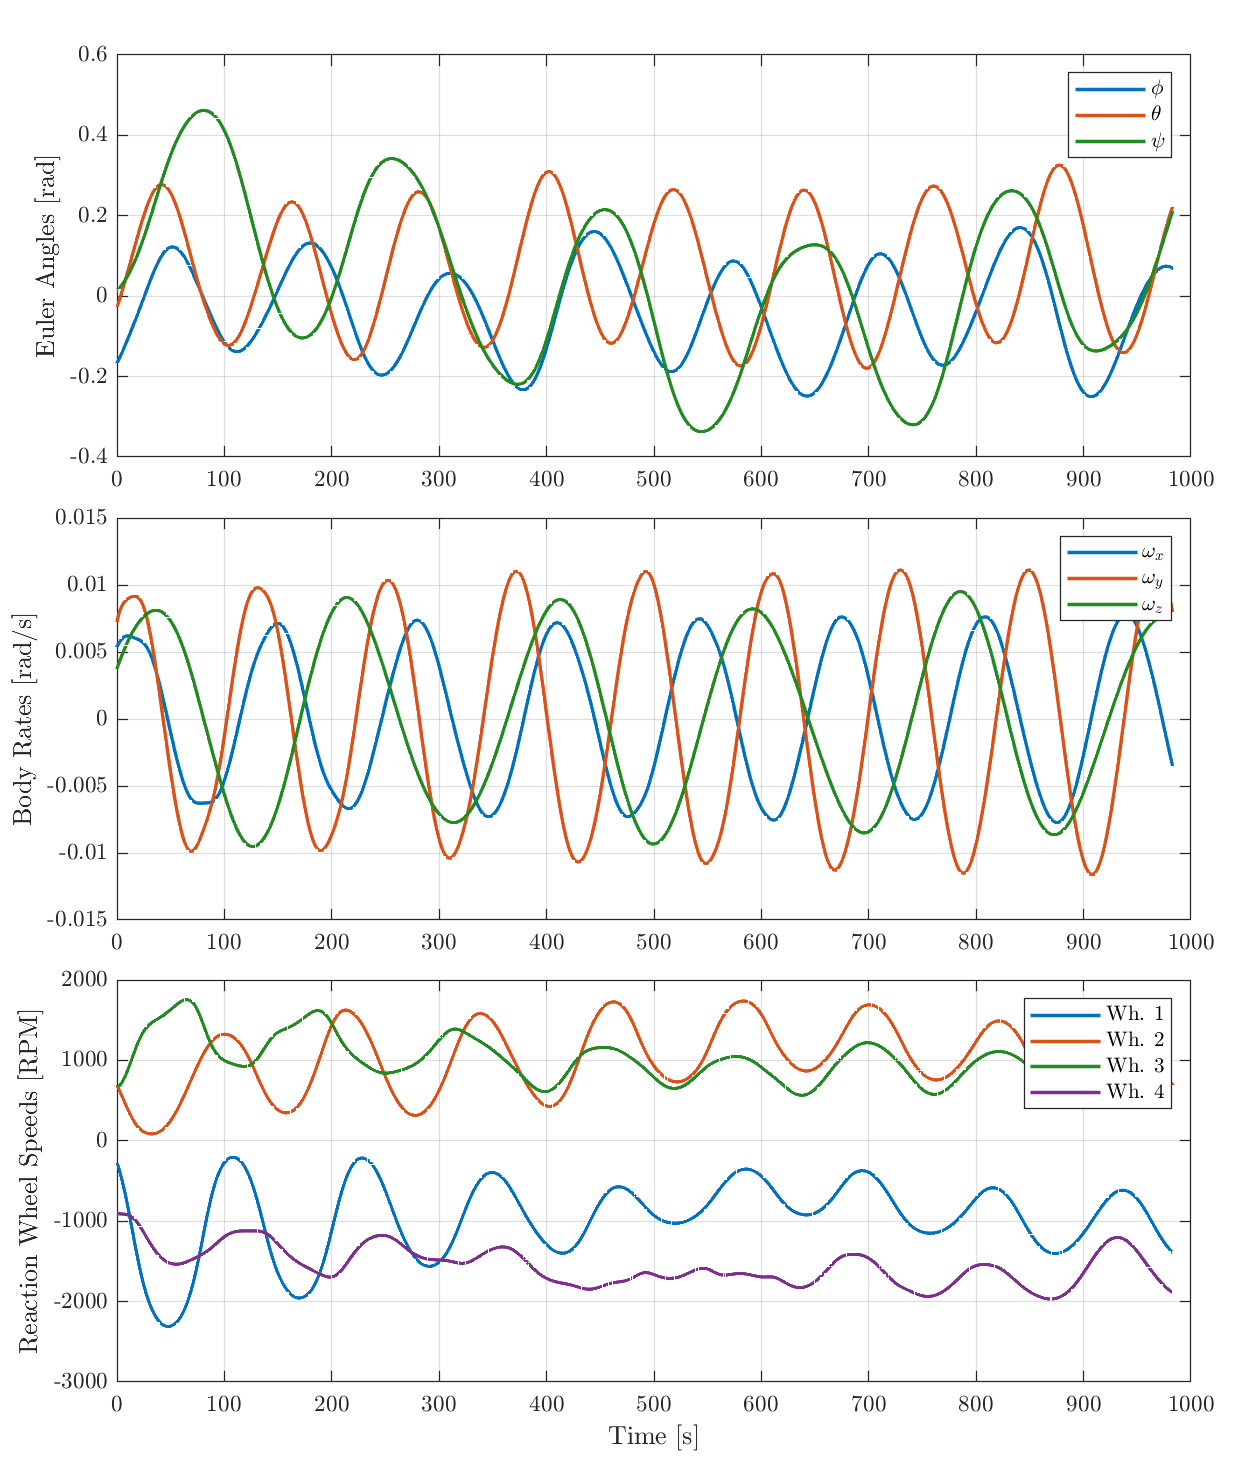
\includegraphics[width=\linewidth]{plots/three_axis_sim_excitation.png}
    \caption{Simulated platform excitation for 3-axis adaptive control}
\end{figure}

\begin{figure}[!ht]
  \centering
  \begin{subfigure}[t]{0.47\textwidth}
    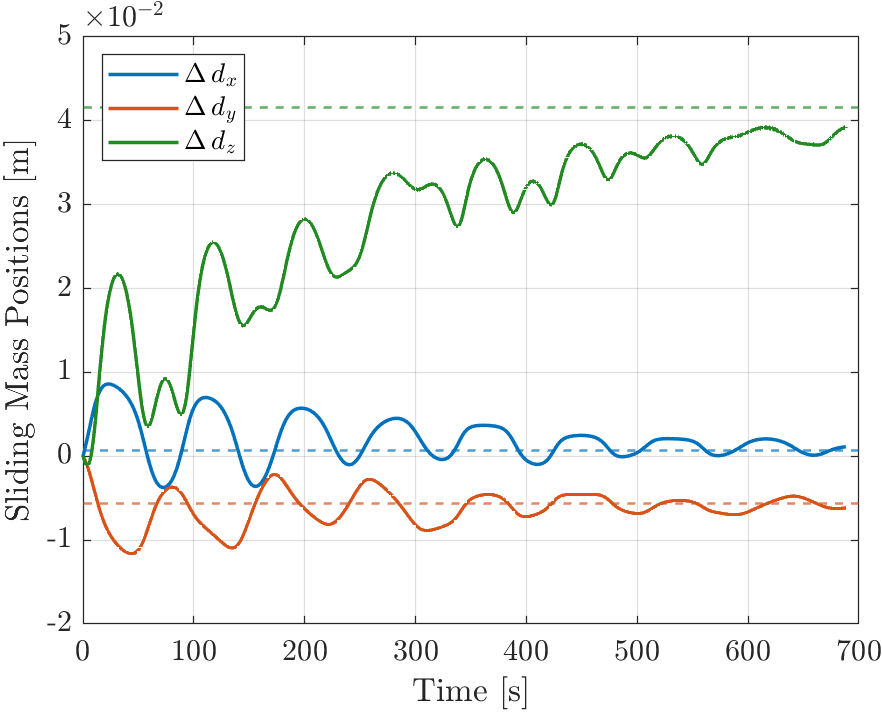
\includegraphics[width=\linewidth]{plots/three_axis_sim_positions_1.png}
    \caption{1st iteration}\label{fig:a}
  \end{subfigure}\hfill
  \begin{subfigure}[t]{0.47\textwidth}
    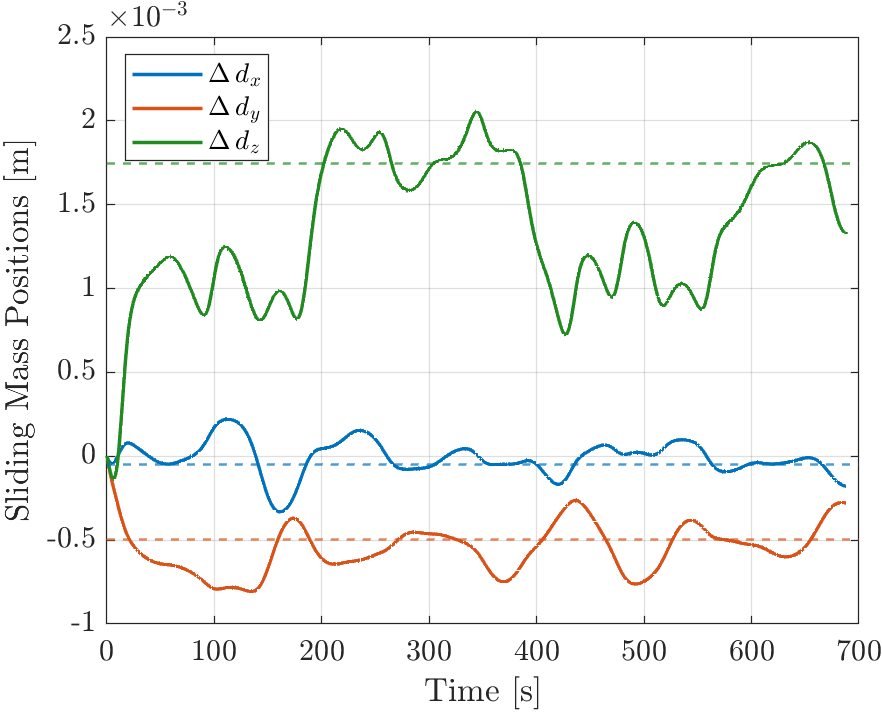
\includegraphics[width=\linewidth]{plots/three_axis_sim_positions_2.png}
    \caption{2nd iteration}\label{fig:b}
  \end{subfigure}
  \caption{Simulated sliding mass positions during 3-axis adaptive control}
  \label{fig:LSR_hardware_iterations}
\end{figure}

\iffalse
Results PID:
horizontal: 2.5e-5
verit 6.7e-7

Results Batch:
horizontal: 1e-7
vert: 2.2e-7

Results UKF
r_z = 6.784e-07

Results 3-axis
horizontal: 4.8261e-06
vertical: 9.7241e-05
\fi